\section{Objective}
\begin{itemize}
	\item To design, construct, and verify a full-wave bridge rectifier circuit on a solderless breadboard using four silicon p-n junction diodes.
	\item To evaluate cycle-by-cycle conduction characteristics during both positive and negative half-cycles of an input AC signal.
	\item To observe, capture, and compare input and output voltage waveforms utilizing a Digital Storage Oscilloscope (DSO).
	\item To compute essential operating metrics including average DC output voltage ($V_{DC}$), RMS output voltage ($V_{rms}$), ripple factor ($r$), and rectification efficiency ($\eta$).
	\item To examine output voltage waveform smoothing using a parallel capacitive filter and compare empirical observations against theoretical predictions.
\end{itemize}

\section{Introduction}
Electronic devices demand a steady direct current (DC) power source for consistent operations, whereas commercial power distribution networks deliver alternating current (AC). Rectifier circuits convert bidirectional alternating signals into unidirectional pulsating outputs. Among fundamental rectifier configurations, the full-wave bridge topology is widely preferred due to its ability to utilize both half-cycles of the AC input without requiring a center-tapped transformer. Constructing the bridge configuration with four diodes arranged in a closed loop ensures continuous current flow across the load resistor in a single direction regardless of input polarity. Since unfiltered rectified outputs retain significant voltage ripple, this experiment further investigates the smoothing capabilities of a parallel reservoir filter capacitor.

\section{Theory}

\subsection{Cycle-by-Cycle Conduction Analysis}
Consider an AC voltage source supplying the bridge rectifier, defined mathematically as:
\[
v_s(t) = V_m \sin(\omega t),
\]
where $V_m = V_{rms}\sqrt{2}$ denotes the peak secondary voltage and $\omega = 2\pi f$ represents the angular frequency.
\begin{itemize}
	\item \textbf{Positive Half-Cycle ($0 < \omega t < \pi$):} The upper secondary terminal operates at a higher potential relative to the lower terminal. Diodes $D_1$ and $D_4$ become forward-biased and conduct, whereas $D_2$ and $D_3$ remain reverse-biased (acting as open switches). Current flows from the source through $D_1$, passes top-to-bottom across load $R_L$, and returns via $D_4$.
	\item \textbf{Negative Half-Cycle ($\pi < \omega t < 2\pi$):} As input polarity reverses, $D_2$ and $D_3$ transition to forward-bias conduction while $D_1$ and $D_4$ become reverse-biased. The current path routes through $D_2$, flows across load $R_L$ in the identical direction, and completes the loop via $D_3$.
\end{itemize}
Because current passes through the load in the same direction across both half-cycles, the output frequency doubles relative to the input line frequency: $f_{\text{out}} = 2 f_{\text{in}}$.

\subsection{Mathematical Formulation of Rectifier Parameters}
Since two diodes conduct concurrently in each half-cycle, their combined forward voltage drops ($V_D \approx \qty{0.7}{\volt}$ per diode) reduce the peak output voltage:
\[
V_{mo} = V_m - 2V_D.
\]
Standard mathematical formulations yield the DC (average) and RMS output voltage values:
\[
V_{DC} = \frac{2V_{mo}}{\pi}, \qquad V_{rms} = \frac{V_{mo}}{\sqrt{2}}.
\]
The ripple factor measures residual AC fluctuations riding on the DC component. For an unfiltered full-wave rectifier:
\[
r = \sqrt{\left(\frac{V_{rms}}{V_{DC}}\right)^2 - 1} = \sqrt{\left(\frac{\pi}{2\sqrt{2}}\right)^2-1} \approx 0.482.
\]
The conversion efficiency $\eta$ and Peak Inverse Voltage (PIV) ratings are expressed as:
\[
\eta = \frac{P_{DC}}{P_{AC}}\times100\%, \qquad \eta_{\max} = \frac{8}{\pi^2}\approx81.2\%, \qquad \text{PIV} = V_m.
\]

\subsection{Effect of a Capacitive Filter}
Connecting a filter capacitor $C$ in parallel with load $R_L$ reduces output ripple voltage. The capacitor charges rapidly to $V_{mo}$ during input peaks and discharges slowly through $R_L$ during conduction off-times. Assuming a linear discharge path, peak-to-peak ripple voltage $V_{r(p\text{-}p)}$ and ripple factor $r$ follow:
\[
V_{r(p\text{-}p)} \approx \frac{I_{DC}}{2fC} = \frac{V_{DC}}{2fR_LC}, \qquad r \approx \frac{1}{4\sqrt{3}\,fR_LC}.
\]
Increasing load resistance $R_L$ or capacitance $C$ minimizes output voltage fluctuations, improving overall power delivery stability.

\section{Apparatus and Components}
\begin{table}[h!]
	\centering
	\caption{List of Equipment and Components Used}
	\vspace{2mm}
	\resizebox{\textwidth}{!}{%
		\begin{tabular}{llc}
			\toprule
			\rowcolor{blue!15}
			\textbf{Item Description} & \textbf{Specification / Rating} & \textbf{Quantity} \\
			\midrule
			Function Generator & Sine wave, \qty{50}{\hertz}, measured peak output \qty{6}{\volt} & 1 \\
			Silicon Rectifier Diodes & 1N4007 & 4 \\
			Load Resistor $R_L$ & \qty{965}{\ohm} & 1 \\
			Electrolytic Filter Capacitor $C$ & \qty{47}{\micro\farad} & 1 \\
			Dual-Channel Digital Storage Oscilloscope (DSO) & With $10\times$ probes & 1 \\
			Solderless Breadboard & Standard Tie-Point & 1 \\
			Connecting Wires & Jumper Wires & As required \\
			\bottomrule
		\end{tabular}%
	}
	\label{tab:apparatus6}
\end{table}

\section{Circuit Diagram}
\begin{figure}[h!]
	\centering
	\begin{circuitikz}[american, scale=0.85]
		\draw (-2,0) to[sV, l=$v_s(t)$] (-2,4);
		\node at (-2,-0.6) [below] {Function Generator};
		\draw (-2,4) -- (0,4) -- (0,2);
		\draw (-2,0) -- (-2,-3) -- (6,-3) -- (6,2);
		\coordinate (L) at (0,2);
		\coordinate (R) at (6,2);
		\coordinate (T) at (3,5);
		\coordinate (Bt) at (3,-1);
		\draw (L) to[D, l=$D_1$] (T);
		\draw (R) to[D, l=$D_2$] (T);
		\draw (Bt) to[D, l=$D_3$] (L);
		\draw (Bt) to[D, l=$D_4$] (R);
		\draw (T) to[R, l=$R_L$] (Bt);
		\draw (T) -- (4.5,5) to[C, l=$C$] (4.5,-1) -- (Bt);
		\draw (Bt) node[ground]{};
		\node at (0,2.4) [above left] {AC$_1$};
		\node at (6,2.4) [above right] {AC$_2$};
		\node at (3,5.4) [above] {$+$ (DC Output)};
	\end{circuitikz}
	\caption{Full-wave bridge rectifier circuit driven by an AC source with parallel load $R_L$ and optional capacitor filter $C$.}
	\label{fig:bridgerectifier}
\end{figure}

\section{Experimental Procedure}
\begin{enumerate}
	\item \textbf{Bridge Assembly:} Mount four 1N4007 diodes on the breadboard following the bridge orientation shown in Figure~\ref{fig:bridgerectifier}, verifying correct terminal polarity.
	\item \textbf{Source Integration:} Connect function generator leads across nodes $\text{AC}_1$ and $\text{AC}_2$, configured to deliver a \qty{50}{\hertz} sinusoidal voltage waveform.
	\item \textbf{Unfiltered Baseline Testing:} Attach load resistor $R_L=\qty{965}{\ohm}$ across output terminals. Display input and output waveforms on DSO Channels 1 and 2 to record peak levels $V_m$ and $V_{mo}$. Derive dependent parameters ($V_{DC}$, $V_{rms}$, $r$, $\eta$) using analytical relationships.
	\item \textbf{Filtered Analysis:} Connect electrolytic capacitor $C=\qty{47}{\micro\farad}$ across load $R_L$, observing waveform smoothing on the DSO. Determine filtered $V_{DC}$ and ripple $V_{r(p\text{-}p)}$ values.
\end{enumerate}

\section{Theoretical Calculation}
Using measured laboratory parameter values ($V_m=\qty{6}{\volt}$, $V_D=\qty{0.7}{\volt}$, $f=\qty{50}{\hertz}$, and $R_L=\qty{965}{\ohm}$):
\[
V_{mo} = V_m - 2V_D = 6 - 1.4 = \qty{4.60}{\volt},
\]
\[
V_{DC} = \frac{2V_{mo}}{\pi} = \frac{2\times4.60}{3.1416} = \qty{2.928}{\volt}, \qquad
I_{DC} = \frac{V_{DC}}{R_L} = \frac{2.928}{965} = \qty{3.03}{\milli\ampere},
\]
\[
V_{rms(\text{out})} = \frac{V_{mo}}{\sqrt{2}} = \frac{4.60}{1.4142} = \qty{3.253}{\volt},
\]
\[
\eta = \frac{V_{DC}^2/R_L}{V_{rms(\text{out})}^2/R_L}\times100\% = \frac{2.928^2}{3.253^2}\times100\% \approx 81.0\%, \qquad \text{PIV} = V_m = \qty{6}{\volt}.
\]
Introducing the \qty{47}{\micro\farad} filter capacitor yields expected peak-to-peak ripple voltage:
\[
V_{r(p\text{-}p)} \approx \frac{V_{DC}}{2fR_LC} = \frac{2.928}{2\times50\times965\times47\times10^{-6}} \approx \qty{0.646}{\volt}.
\]

\section{Data Collection}
\label{sec:datacollection6}

\begin{table}[h!]
	\centering
	\caption{Unfiltered Rectifier Performance}
	\vspace{2mm}
	\resizebox{\textwidth}{!}{%
		\begin{tabular}{ccccccc}
			\toprule
			\rowcolor{blue!15}
			\textbf{Load $R_L$} & \textbf{Peak Input $V_m$} & \textbf{Peak Output $V_{mo}$} & \textbf{Measured $V_{DC}$} & \textbf{Measured $V_{rms}$} & \textbf{Ripple Factor $r$} & \textbf{Efficiency $\eta$} \\
			\midrule
			\qty{965}{\ohm} & \qty{6}{\volt} & \qty{2}{\volt} & \qty{1.27}{\volt} & \qty{1.41}{\volt} & 0.483 & 81.1\% \\
			\bottomrule
		\end{tabular}%
	}
	\label{tab:unfiltereddata6}
\end{table}

\begin{table}[h!]
	\centering
	\caption{Filtered Rectifier Performance: Effect of the \qty{47}{\micro\farad} Capacitor}
	\vspace{2mm}
	\begin{tabular}{cccc}
		\toprule
		\rowcolor{blue!15}
		\textbf{Load $R_L$} & \textbf{Filter $C$} & \textbf{Measured $V_{DC}$} & \textbf{Ripple $V_{r(p\text{-}p)}$} \\
		\midrule
		\qty{965}{\ohm} & \qty{47}{\micro\farad} & \qty{1.78}{\volt} & \qty{0.44}{\volt} \\
		\bottomrule
	\end{tabular}
	\label{tab:filtereddata6}
\end{table}

\subsection{Oscilloscope Waveforms}

\begin{figure}[h!]
	\centering
	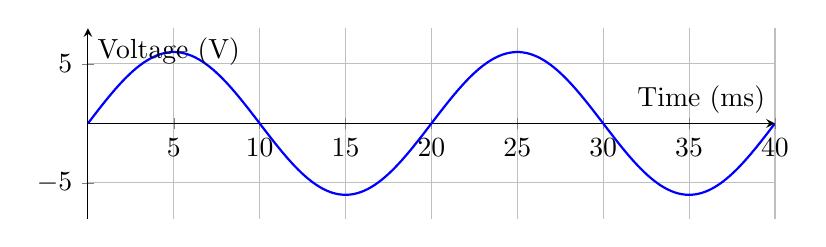
\begin{tikzpicture}
		\begin{axis}[
			width=0.85\textwidth,
			height=4cm,
			xlabel={Time (ms)},
			ylabel={Voltage (V)},
			xmin=0, xmax=40,
			ymin=-8, ymax=8,
			axis lines=middle,
			grid=major,
			]
			\addplot[domain=0:40, samples=200, thick, blue] {6*sin(x/20*360)};
		\end{axis}
	\end{tikzpicture}
	\caption{Sinusoidal AC input voltage trace ($V_m=\qty{6}{\volt}$, $f=\qty{50}{\hertz}$).}
	\label{fig:waveinput6}
\end{figure}

\begin{figure}[h!]
	\centering
	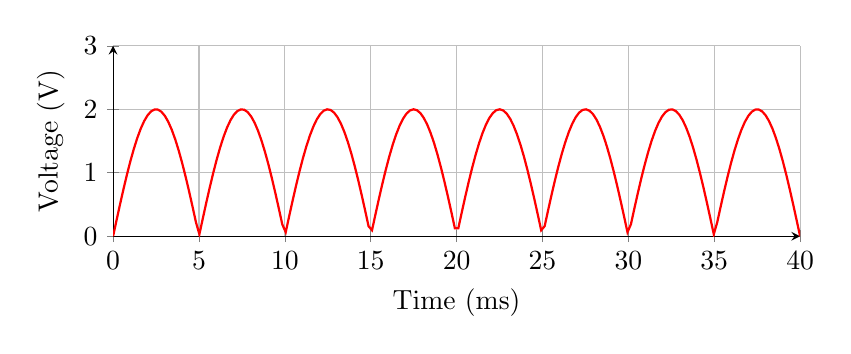
\begin{tikzpicture}
		\begin{axis}[
			width=0.85\textwidth,
			height=4cm,
			xlabel={Time (ms)},
			ylabel={Voltage (V)},
			xmin=0, xmax=40,
			ymin=0, ymax=3,
			axis lines=left,
			grid=major,
			]
			\addplot[domain=0:40, samples=200, thick, red] {2*abs(sin(x/10*360))};
		\end{axis}
	\end{tikzpicture}
	\caption{Unfiltered full-wave rectified output voltage trace ($V_{mo}=\qty{2}{\volt}$, $f=\qty{100}{\hertz}$).}
	\label{fig:waveoutput6}
\end{figure}

\begin{figure}[h!]
	\centering
	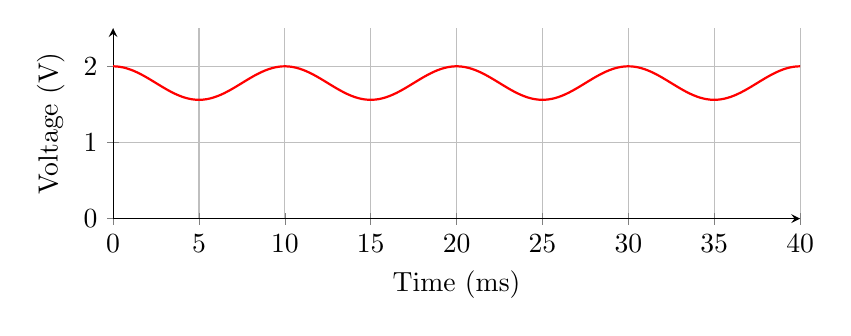
\begin{tikzpicture}
		\begin{axis}[
			width=0.85\textwidth,
			height=4cm,
			xlabel={Time (ms)},
			ylabel={Voltage (V)},
			xmin=0, xmax=40,
			ymin=0, ymax=2.5,
			axis lines=left,
			grid=major,
			]
			\addplot[domain=0:40, samples=200, thick, red] {1.78+0.22*cos(x/10*360)};
		\end{axis}
	\end{tikzpicture}
	\caption{Filtered DC output voltage trace demonstrating smoothed output waveform.}
	\label{fig:wavefiltered6}
\end{figure}

\section{Result Analysis}
\label{sec:resultanalysis6}
Experimental measurement yielded a peak output voltage of $V_{mo}=\qty{2}{\volt}$, exhibiting a variance relative to theoretical calculations (\qty{4.60}{\volt}). Dimensionless shape parameters aligned closely with theoretical predictions: the observed ripple factor ($0.483$) matched theoretical limits ($0.482$), while efficiency reached $81.1\%$ against an ideal maximum of $81.2\%$. Adding the \qty{47}{\micro\farad} filter capacitor increased $V_{DC}$ from \qty{1.27}{\volt} to \qty{1.78}{\volt} while attenuating peak-to-peak ripple to \qty{0.44}{\volt}, confirming successful waveform filtering.

\section{Conclusion}
The full-wave bridge rectifier circuit was constructed and evaluated under AC excitation ($V_m=\qty{6}{\volt}$, $f=\qty{50}{\hertz}$). Full-wave rectification was successfully verified through comparative waveform measurements and quantitative parameter evaluation. Adding a parallel filter capacitor effectively smoothed voltage variations, elevating average DC output voltage while reducing ripple components.

\section{References}
\begin{tcolorbox}[colback=gray!5, colframe=gray!40, arc=2mm]
	\begin{enumerate}
		\item Boylestad, R. L., \& Nashelsky, L. (2013). \textit{Electronic Devices and Circuit Theory} (11th ed.). Pearson.
		\item Alexander, C. K., \& Sadiku, M. N. O. (2016). \textit{Fundamentals of Electric Circuits} (6th ed.). McGraw-Hill Education.
		\item Sedra, A. S., \& Smith, K. C. (2014). \textit{Microelectronic Circuits} (7th ed.). Oxford University Press.
	\end{enumerate}
\end{tcolorbox}